%% LyX 2.3.6.1 created this file.  For more info, see http://www.lyx.org/.
%% Do not edit unless you really know what you are doing.
\documentclass[12pt,preprint,3p]{elsarticle}
\usepackage[latin9]{inputenc}
\usepackage{float}
\usepackage{textcomp}
\usepackage{amsmath}
\usepackage{amssymb}
\usepackage{graphicx}

\makeatletter

%%%%%%%%%%%%%%%%%%%%%%%%%%%%%% LyX specific LaTeX commands.
%% Because html converters don't know tabularnewline
\providecommand{\tabularnewline}{\\}

%%%%%%%%%%%%%%%%%%%%%%%%%%%%%% User specified LaTeX commands.
%%
%% Copyright 2007, 2008, 2009 Elsevier Ltd
%%
%% This file is part of the 'Elsarticle Bundle'.
%% ---------------------------------------------
%%
%% It may be distributed under the conditions of the LaTeX Project Public
%% License, either version 1.2 of this license or (at your option) any
%% later version.  The latest version of this license is in
%%    http://www.latex-project.org/lppl.txt
%% and version 1.2 or later is part of all distributions of LaTeX
%% version 1999/12/01 or later.
%%
%% The list of all files belonging to the 'Elsarticle Bundle' is
%% given in the file `manifest.txt'.
%%

%% Template article for Elsevier's document class `elsarticle'
%% with numbered style bibliographic references
%% SP 2008/03/01
%%
%%
%%
%% $Id: elsarticle-template-num.tex 4 2009-10-24 08:22:58Z rishi $
%%
%%


%% Use the option review to obtain double line spacing
%% \documentclass[preprint,review,12pt]{elsarticle}

%% Use the options 1p,twocolumn; 3p; 3p,twocolumn; 5p; or 5p,twocolumn
%% for a journal layout:
%% \documentclass[final,1p,times]{elsarticle}
%% \documentclass[final,1p,times,twocolumn]{elsarticle}
%% \documentclass[final,3p,times]{elsarticle}
%% \documentclass[final,3p,times,twocolumn]{elsarticle}
%% \documentclass[final,5p,times]{elsarticle}
%% \documentclass[final,5p,times,twocolumn]{elsarticle}

%% if you use PostScript figures in your article
%% use the graphics package for simple commands
%% \usepackage{graphics}
%% or use the graphicx package for more complicated commands
%% \usepackage{graphicx}
%% or use the epsfig package if you prefer to use the old commands
%% \usepackage{epsfig}

%% The amssymb package provides various useful mathematical symbols
%% The amsthm package provides extended theorem environments
%% \usepackage{amsthm}

%% The lineno packages adds line numbers. Start line numbering with
%% \begin{linenumbers}, end it with \end{linenumbers}. Or switch it on
%% for the whole article with \linenumbers after \end{frontmatter}.
%% \usepackage{lineno}

%% natbib.sty is loaded by default. However, natbib options can be
%% provided with \biboptions{...} command. Following options are
%% valid:

%%   round  -  round parentheses are used (default)
%%   square -  square brackets are used   [option]
%%   curly  -  curly braces are used      {option}
%%   angle  -  angle brackets are used    <option>
%%   semicolon  -  multiple citations separated by semi-colon
%%   colon  - same as semicolon, an earlier confusion
%%   comma  -  separated by comma
%%   numbers-  selects numerical citations
%%   super  -  numerical citations as superscripts
%%   sort   -  sorts multiple citations according to order in ref. list
%%   sort&compress   -  like sort, but also compresses numerical citations
%%   compress - compresses without sorting
%%
%% \biboptions{comma,round}

% \biboptions{}


%\journal{Nuclear Physics B}

\makeatother

\begin{document}

\part{Implementation and Technical Data}

\section{Modeling of fuel cell}

\subsection{Governing equations}

For this model the current is split into an ionic and electronic part.
Protons flow through the membrane and form an ionic current. The electrons
only flow through the solid matrix of electrodes, resulting in an
electronic current. Therefore, it satisfies the following proton potential
equation \citep{he_huang_sun_wang_2013}

\begin{align}
\nabla\cdot(-\sigma_{\textrm{s}}\nabla\phi_{\textrm{s}}) & =\text{\ensuremath{S}}_{\textrm{s}}\\
\nabla\cdot(-\sigma_{\textrm{m}}\nabla\phi_{\textrm{m}}) & =\text{\ensuremath{S}}_{\textrm{m}}
\end{align}
where $\phi_{\textrm{s}}$ and $\phi_{\textrm{m}}$ are the protonic
and electronic potential. The electronic conductivity is listed in
Table \ref{tab:Model-parameters}, the protonic conductivity in electrolyte
$\sigma_{\textrm{s}}$ is given by \citep{he_huang_sun_wang_2013}

\begin{equation}
\sigma_{\textrm{s}}=\frac{1}{2}\left(0.5139\lambda-0.326\right)\exp\left[1268\left(\frac{1}{303}-\frac{1}{T}\right)\right]
\end{equation}

and in porous electrode the protonic conductivity is

\begin{equation}
\sigma_{\textrm{PE}}=\varepsilon_{\textrm{cm}}^{1.5}\sigma_{\textrm{s}}.
\end{equation}

$S$ is the current source term and defined as
\begin{center}
anode catalyst layer:
\begin{equation}
S_{\textrm{m}}=j_{\textrm{a}}\,\,\,S_{\textrm{s}}=\text{\textminus}j_{\textrm{a}}
\end{equation}
\par\end{center}

\begin{center}
cathode catalyst layer:
\begin{equation}
S_{\textrm{m}}=j_{\textrm{c}}\,\,\,S_{\textrm{s}}=\text{\textminus}j_{\textrm{c}}
\end{equation}
\par\end{center}

\begin{flushleft}
The source terms in both species and charge equations are related
to the transfer current density $j_{a}$ and $j_{c}$, which was calculated
by using a simplified Butler--Volmer equation given as
\par\end{flushleft}

\begin{equation}
j_{\textrm{a}}=i_{0\textrm{a}}r_{\textrm{a}}\left(\frac{C_{\textrm{H}_{2}}}{C_{\textrm{\ensuremath{\textrm{H}_{2}},ref}}}\right)^{0.5}\left(\frac{\alpha_{\textrm{a}}+\alpha_{\textrm{c}}}{RT}F\eta_{\textrm{a}}\right)
\end{equation}

\begin{equation}
j_{\textrm{c}}=i_{0\textrm{c}}r_{\textrm{c}}\left(\frac{C_{\textrm{O}_{2}}}{C_{\textrm{\ensuremath{\textrm{O}_{2}},ref}}}\right)\exp\left(-\frac{\alpha_{\textrm{c}}}{RT}F\eta_{\textrm{c}}\right)
\end{equation}

\begin{flushleft}
where $\eta$ represents the potential difference between solid matrix
and electrolyte and is defined as
\par\end{flushleft}

\begin{center}
anode side:
\begin{equation}
\eta_{\textrm{a}}=\phi_{\textrm{s}}-\phi_{\textrm{m}}
\end{equation}
\par\end{center}

\begin{center}
cathode side:
\begin{equation}
\eta_{\textrm{c}}=\phi_{\textrm{s}}-\phi_{\textrm{m}}-V_{\textrm{OC}}
\end{equation}
\par\end{center}

\subsection{Fuel cell setup}

PEMFC consists of gas diffusion layers, porous electrode layers at
anode and cathode side and the membrane in between \citep{Ubong2009}. 

\begin{figure}[H]
\centering{}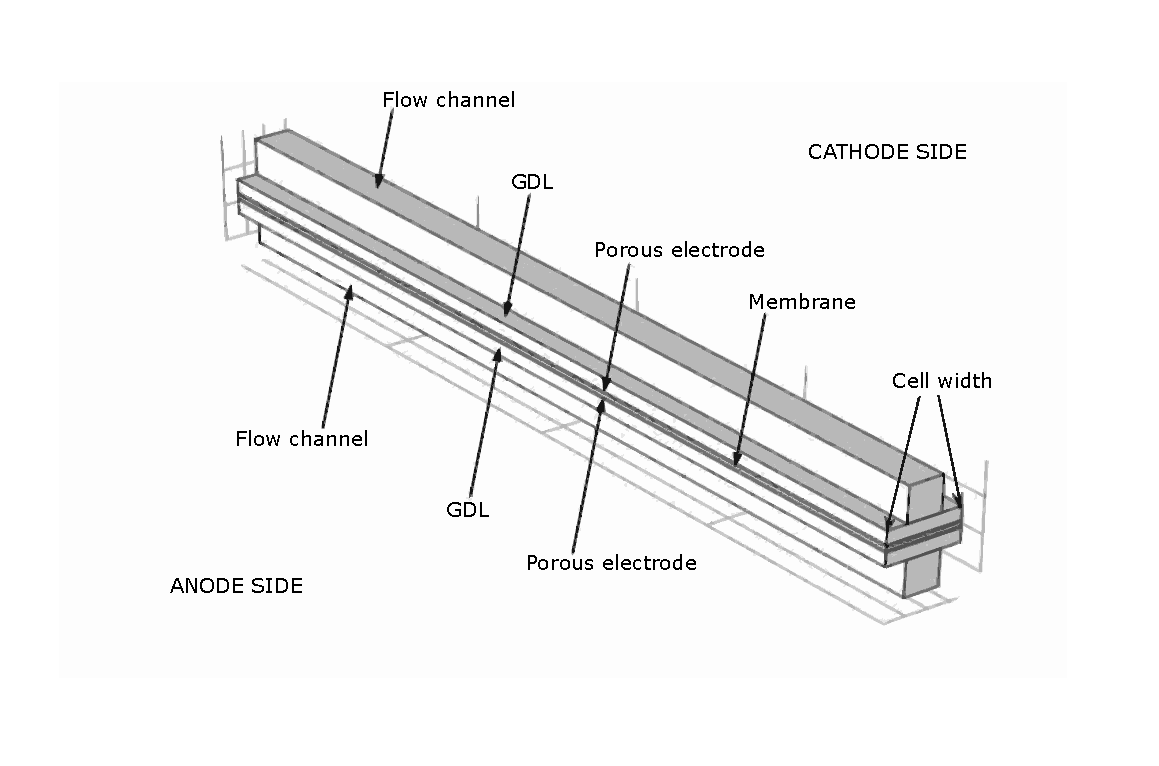
\includegraphics[scale=0.7]{images/Geometry-of-fuel-cell_inkscape}\caption{Geometry of the fuel cell model \citep{Ubong2009}}
\end{figure}

\begin{flushleft}
The coefficients are described in Table~\ref{tab:Model-parameters}.
\par\end{flushleft}

\begin{table}[H]
\caption{Model parameters and values\label{tab:Model-parameters}}
\begin{tabular}{lcccccc}
 &  &  &  &  &  & \tabularnewline
\hline 
\hline 
Parameter &  & Symbol &  & Value &  & Unit\tabularnewline
\hline 
\hline 
Cell length &  & $L$ &  & $10^{-2}$ &  & \textsf{$\textrm{m}$}\tabularnewline
Gas diffusion layers (GDL) thickness &  & $H_{gdl}$ &  & $38\times10^{-5}$ &  & m\tabularnewline
Reference hydrogen molar concentration &  & $C_{\textrm{H}_{2},\textrm{ref}}$ &  & $40.88$ &  & $\textrm{mol}/\textrm{m}^{3}$\tabularnewline
Reference oxygen molar concentration &  & $C_{\textrm{O}_{2},\textrm{ref}}$ &  & $40.88$ &  & $\textrm{mol}/\textrm{m}^{3}$\tabularnewline
Electronic conductivity &  & $\sigma_{m}$ &  & $222$ &  & $\textrm{S}/\textrm{m}$\tabularnewline
Exchange current density, anode &  & $i_{0\textrm{a}}$ &  & $1$ &  & $\textrm{A}/\textrm{m}^{2}$\tabularnewline
Exchange current density, cathode &  & $i_{0\textrm{c}}$ &  & $1$ &  & $\textrm{A}/\textrm{m}^{2}$\tabularnewline
Ratio of reaction surface, anode &  & $r_{\textrm{a}}$ &  & $10^{9}$ &  & $1/\mathrm{m}$\tabularnewline
Ratio of reaction surface, cathode &  & $r_{\textrm{c}}$ &  & $10^{4}$ &  & $1/\mathrm{m}$\tabularnewline
Hydrogen concentrations &  & $C_{\textrm{H}_{2}}$ &  & $60$ &  & $\textrm{mol}/\textrm{m}^{3}$\tabularnewline
Oxygen concentrations &  & $C_{\textrm{O}_{2}}$ &  & $10$ &  & $\textrm{mol}/\textrm{m}^{3}$\tabularnewline
Transfer coefficient, anode &  & $\alpha_{\textrm{a}}/\alpha_{\textrm{c}}$ &  & $1/1$ &  & -\tabularnewline
Transfer coefficient, cathode &  & $\alpha_{\textrm{c}}$ &  & 1 &  & -\tabularnewline
Open circuit voltage &  & $V_{\textrm{OC}}$ &  & $1.229$ &  & $\textrm{V}$\tabularnewline
Universal gas constant &  & $R$ &  & $8.31$ &  & $\textrm{J/mol/K}$\tabularnewline
Faraday constant &  & $F$ &  & $96485$ &  & $\textrm{C/mol}$\tabularnewline
 &  &  &  &  &  & \tabularnewline
Cell width &  & $W$ &  & $2\times10^{-3}$ &  & $\textrm{m}$\tabularnewline
Membrane thickness &  & $H_{\textrm{mem}}$ &  & $100\times10^{-6}$ &  & $\textrm{m}$\tabularnewline
Porous electrode thickness &  & $H_{\textrm{el}}$ &  & $50\times10^{-6}$ &  & $\textrm{m}$\tabularnewline
Electrolyte phase volume fraction &  & $\varepsilon_{\textrm{cm}}$ &  & $1$ &  & -\tabularnewline
Water content &  & $\lambda$ &  & $5$ &  & -\tabularnewline
Cell Temperature &  & $T$ &  & $453.15$ &  & $\textrm{K}$\tabularnewline
\hline 
\end{tabular}
\end{table}


\subsection{Variation of operation Fuel cell parameters}

The average cell power density is one of the most significant magnitudes
of fuel cells whose increase is of paramount importance. The Fig.
\ref{fig:Variation-of-geometry} shows the plot of average cell power
density depending on the required voltage for different geometry parameters
like cell width $\left[W\right]$, membrane thickness $\left[H_{\textrm{mem}}\right]$
and porous electrode thickness $\left[H_{\textrm{el}}\right]$.
\begin{center}
\begin{figure}[H]
\centering{}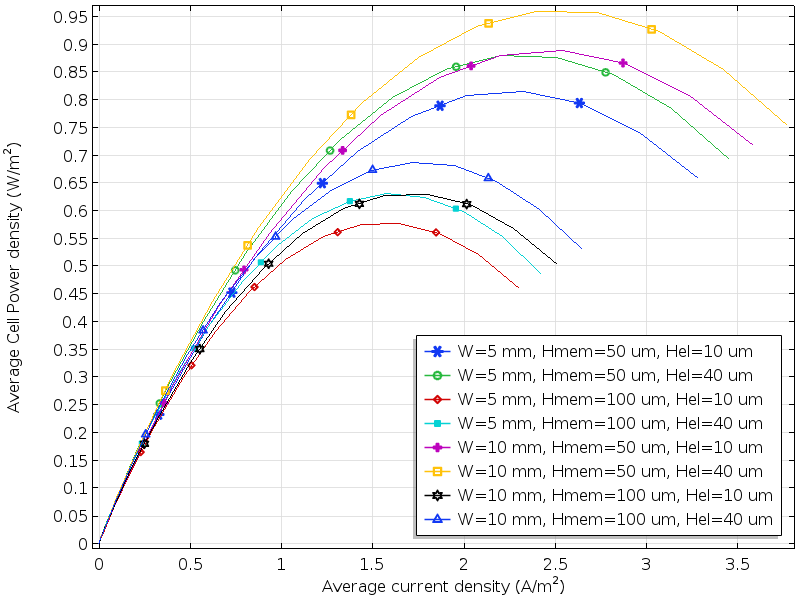
\includegraphics[scale=0.6]{images/CellGeom}\caption{\label{fig:Variation-of-geometry}Variation of geometry parameters}
\end{figure}
\par\end{center}

\begin{flushleft}
The average cell power density is not only depended on cell geometry
but also on other parameters listed in Table \ref{tab:Model-parameters}.
In Fig \ref{fig:Variation-of-some} the average cell power density
is plotted for other varying properties like hydrogen concentrations
$\left[C_{\textrm{H}_{2}}\right]$, oxygen concentrations $\left[C_{\textrm{O}_{2}}\right]$
and the volume fraction of membrane in porous electrode $\left[\varepsilon_{\textrm{cm}}\right]$.
\par\end{flushleft}

\begin{center}
\begin{figure}[H]
\centering{}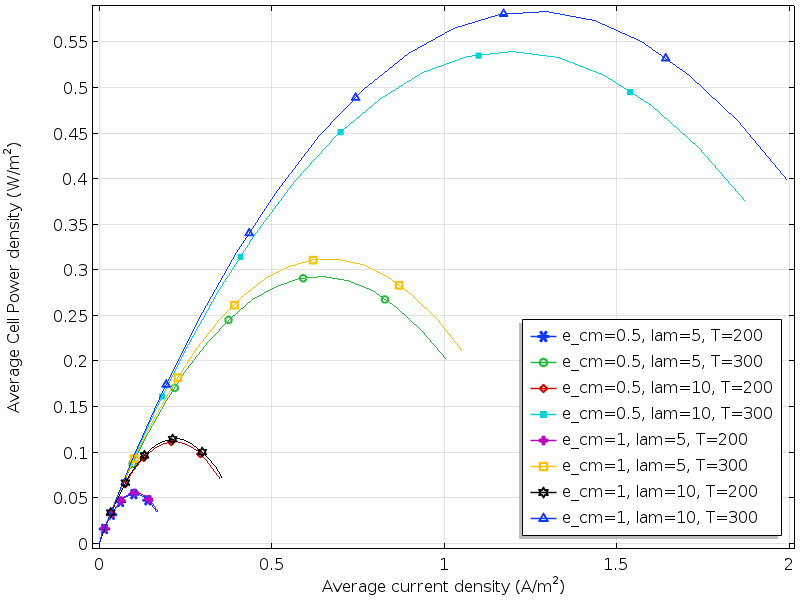
\includegraphics[scale=0.6]{images/CellParam}\caption{\label{fig:Variation-of-some}Variation of some other properties}
\end{figure}
\par\end{center}

\begin{flushleft}
The case is treated where a desired mean cell power density is given
and the task is to find the parameters that achieve this power by
variation. This is an optimization problem, and the genetic algorithm
is used to solve the problem.
\par\end{flushleft}

\subsection{Parameter identification through optimization}

In order to use a genetic algorithm, a solution space must first be
specified. In our case, the following parameters are taken from Table
\ref{tab:Solution-space-for} with a range and the step size is the
resolution of the solution space.
\begin{flushleft}
\begin{table}[H]
\caption{\label{tab:Solution-space-for}Solution space for genetic algorithms}

\centering{}%
\begin{tabular}{lcccccc}
 &  &  &  &  &  & \tabularnewline
\hline 
\hline 
Symbol &  & Range &  & Step size &  & Unit\tabularnewline
\hline 
\hline 
$W$ &  & $\left[\begin{array}{cc}
1 & 10\end{array}\right]$ &  & $0.1$ &  & $\mathrm{mm}$\tabularnewline
$H_{\textrm{mem}}$ &  & $\left[\begin{array}{cc}
10 & 110\end{array}\right]$ &  & $10$ &  & $\mu\mathrm{m}$\tabularnewline
$H_{\textrm{el}}$ &  & $\left[\begin{array}{cc}
10 & 110\end{array}\right]$ &  & $1$ &  & $\mu\mathrm{m}$\tabularnewline
$\varepsilon_{\textrm{cm}}$ &  & $\left[\begin{array}{cc}
0.1 & 1\end{array}\right]$ &  & $0.1$ &  & -\tabularnewline
$\lambda$ &  & $\left[\begin{array}{cc}
1.5 & 15\end{array}\right]$ &  & $1.5$ &  & -\tabularnewline
$T$ &  & $\left[\begin{array}{cc}
200 & 400\end{array}\right]$ &  & $20$ &  & $\mathrm{K}$\tabularnewline
\hline 
\end{tabular}
\end{table}
From the solution space an initial population is randomly generated
which is a set of individuals or chromosomes. The position or locations
in a chromosome are referred to as genes to which individual parameters
are assigned.
\par\end{flushleft}

Since the fitness function is a positive real number, it is obtained
by scaling from the objective function, which corresponds to the optimization
goal of the optimization problem. The objective function that is used
is the average cell power density

\begin{equation}
F_{p}=\sqrt{\overset{N}{\underset{j=1}{\sum}}\left|p_{j}\left(W,H_{\textrm{mem}},...,T\right)-\hat{p}_{j}\right|^{2}}\overset{!}{=}\mathrm{min}
\end{equation}
where $p_{j}$ is the simulated and $\hat{p}_{j}$ the desired average
cell power density. Index $j$ represents various points on the average
cell power density curve where the simulated and desired average cell
power density are compared and evaluated. The number of points is
chosen as N = 21 that means that the output power is evaluated for
21 different required output voltages. .

\section{Modeling of reverberation chamber}

\subsection{Governing equations}

A real life ERC differs from a cavity resonator because it normally
contains one or more stirrers \citep{https://doi.org/10.25673/4794}.
However, due to the simplicity of the model, it is still preferable
to start by analyzing a cavity resonator and later supplement the
model in order to achieve an ERC. Thus, the Helmolz equation is initially
applied to the electric and magnetic fields of the cavity resonator
through

\begin{equation}
\triangle\overset{\rightarrow}{E}(\overset{\rightarrow}{r})+k^{2}\cdot\overset{\rightarrow}{E}(\overset{\rightarrow}{r})=0
\end{equation}

\begin{equation}
\triangle\overset{\rightarrow}{H}(\overset{\rightarrow}{r})+k^{2}\cdot\overset{\rightarrow}{H}(\overset{\rightarrow}{r})=0
\end{equation}

\begin{equation}
k=\frac{\omega}{\sqrt{\varepsilon_{0}\mu_{0}}}
\end{equation}

where $\varepsilon_{0}$ the permittivity and $\mu_{0}$ the permeability
of the medium (air) is in which the wave is propagating. Due to their
almost equal qualities, the permittivity and the permeability for
the vacuum will be used instead of those for air. In addition, it
is assumed that the tangential components of the electric field and
the normal components of the magnetic field on the walls disappear
as seen in

\begin{equation}
\overset{\rightarrow}{n}\times\overset{\rightarrow}{E}=0
\end{equation}

\begin{equation}
\overset{\rightarrow}{n}\cdot\overset{\rightarrow}{H}=0
\end{equation}

\begin{flushleft}
where $\overrightarrow{n}$ is the surface normal vector and the convention
is also used that the z-axis is chosen as the reference direction.
This leads to the discrete solution in the direction of the z-axis
for the electric and magnetic fields with the resonance frequency
\par\end{flushleft}

\begin{equation}
f_{res}=\frac{1}{2}\frac{1}{\sqrt{\varepsilon_{0}\mu_{0}}}k_{xyz}=\frac{1}{2}\frac{1}{\sqrt{\varepsilon_{0}\mu_{0}}}\sqrt{\left(\frac{l}{a}\right)^{2}+\left(\frac{m}{b}\right)^{2}+\left(\frac{n}{c}\right)^{2}}
\end{equation}

\begin{flushleft}
for the number triple $l,m$ and $n$ applies, $l,m=0,1,2,3...$ and
$n=1,2,3...$.
\par\end{flushleft}

\subsection{Reverberation chamber Setup}

An overview of the setup of the aluminium resonance chamber was modeled
and is displayed in Fig.\ref{fig:MVK_set_up}. A mode stirrer and
a Vivaldi antenna - as a transmitting antenna exciting the field inside
the ERC - were placed inside the chamber. The details describing the
geometry and position for each item are listed in Table \ref{tab:Model-parameters-1}.

\begin{figure}[H]
\centering{}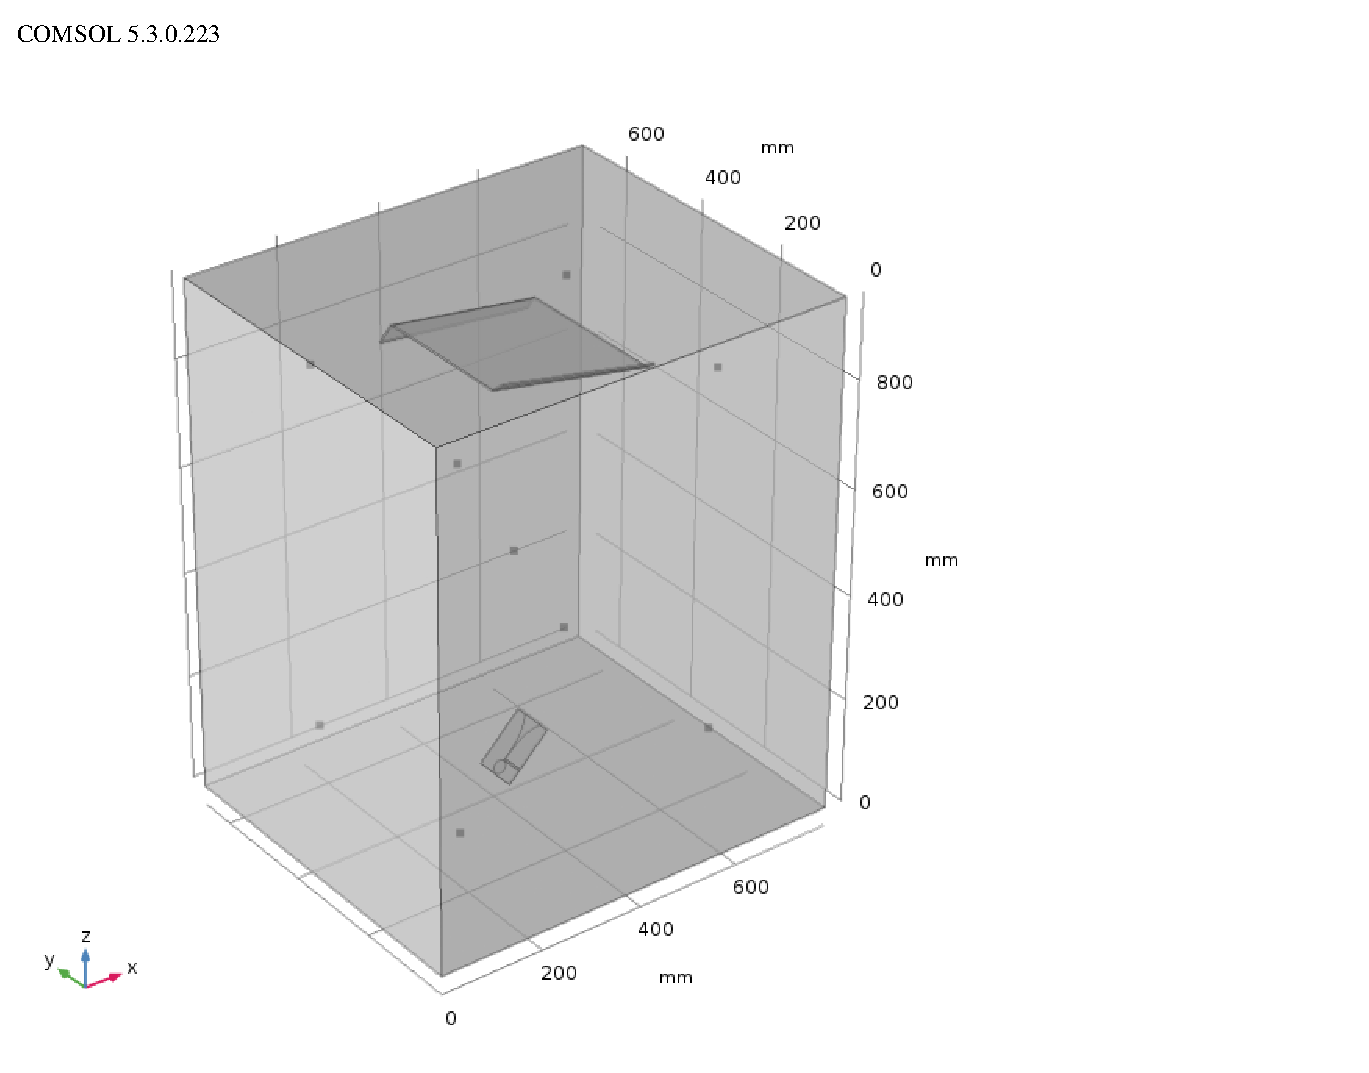
\includegraphics[bb=-67.4737bp 0bp 502.304bp 475bp,clip,scale=0.7]{images/2}\caption{\label{fig:MVK_set_up}Geometry of the resonance chamber, see Table
\ref{tab:Model-parameters-1} for details}
\end{figure}

\begin{flushleft}
A Vivaldi antenna was chosen as the source for the simulation due
to the wideband characteristic. As shown in Fig.\ref{fig:Vivaldi_antenna},
the antenna was positioned in the center of the xy-plane of the chamber
floor with an established angle and height from the chambers floor.
\par\end{flushleft}

\begin{flushleft}
\begin{figure}[H]
\begin{centering}
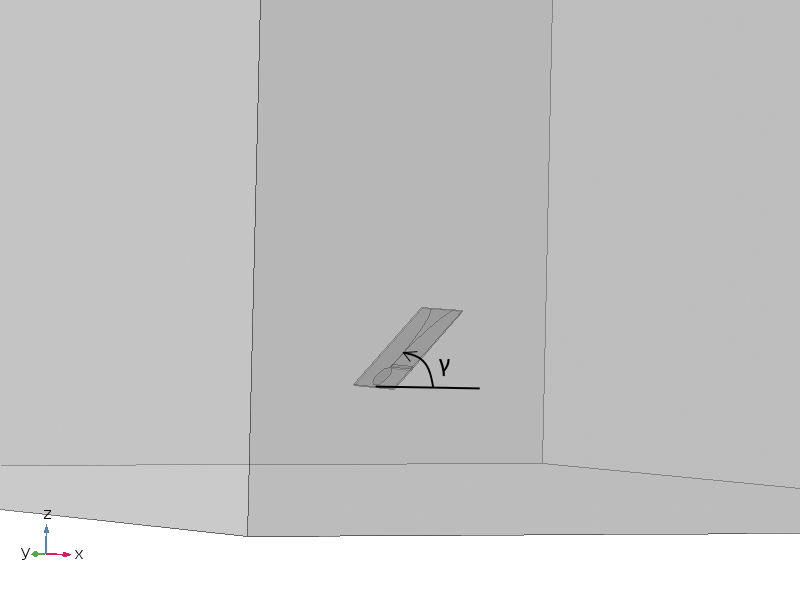
\includegraphics[bb=0bp 0bp 525bp 450bp,clip,scale=0.4]{images/antennaposition1}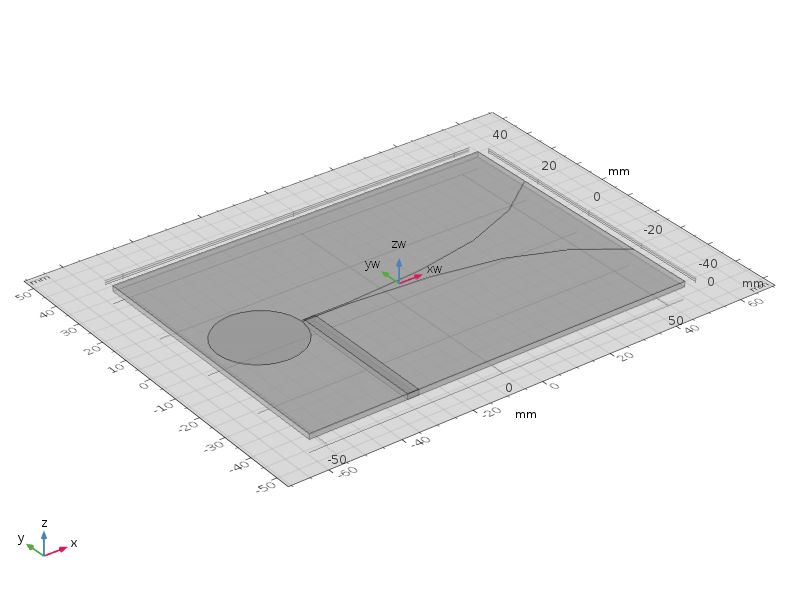
\includegraphics[scale=0.4]{images/antenna1}
\par\end{centering}
\centering{}\caption{\label{fig:Vivaldi_antenna}Vivaldi antenna geometry and position,
see Table \ref{tab:Model-parameters-1}}
\end{figure}
Fig.\ref{fig: Stirrer_geometry} shows a close up view of the stirrer
and specifies the angle of the stirrer wings, the distances of the
wings, and the length and width of the stirrer. Significant parameters
this work will be concerned with are distances $tr_{1}y_{1}$, $tr_{1}y_{2}$,
$tr_{2}y_{1}$, and $tr_{2}y_{2}$ which correspond to the distance
of the wing edges from the boundary of the stirrer length $St_{L}=0$
mm. 
\par\end{flushleft}

\begin{flushleft}
\begin{figure}[H]
\noindent \begin{centering}
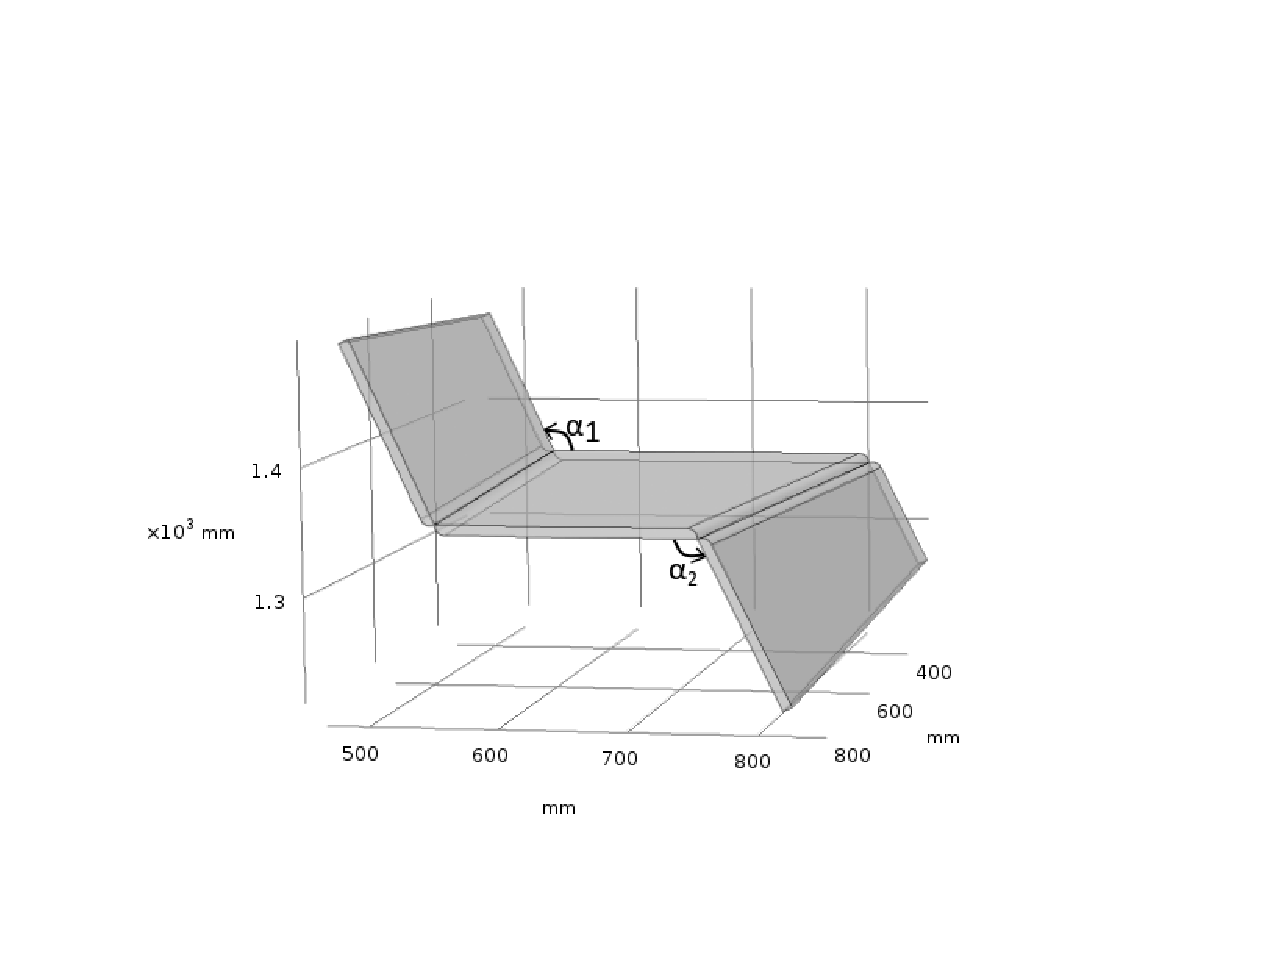
\includegraphics[bb=60bp 0bp 465bp 450bp,clip,scale=0.55]{images/stirrer_view1}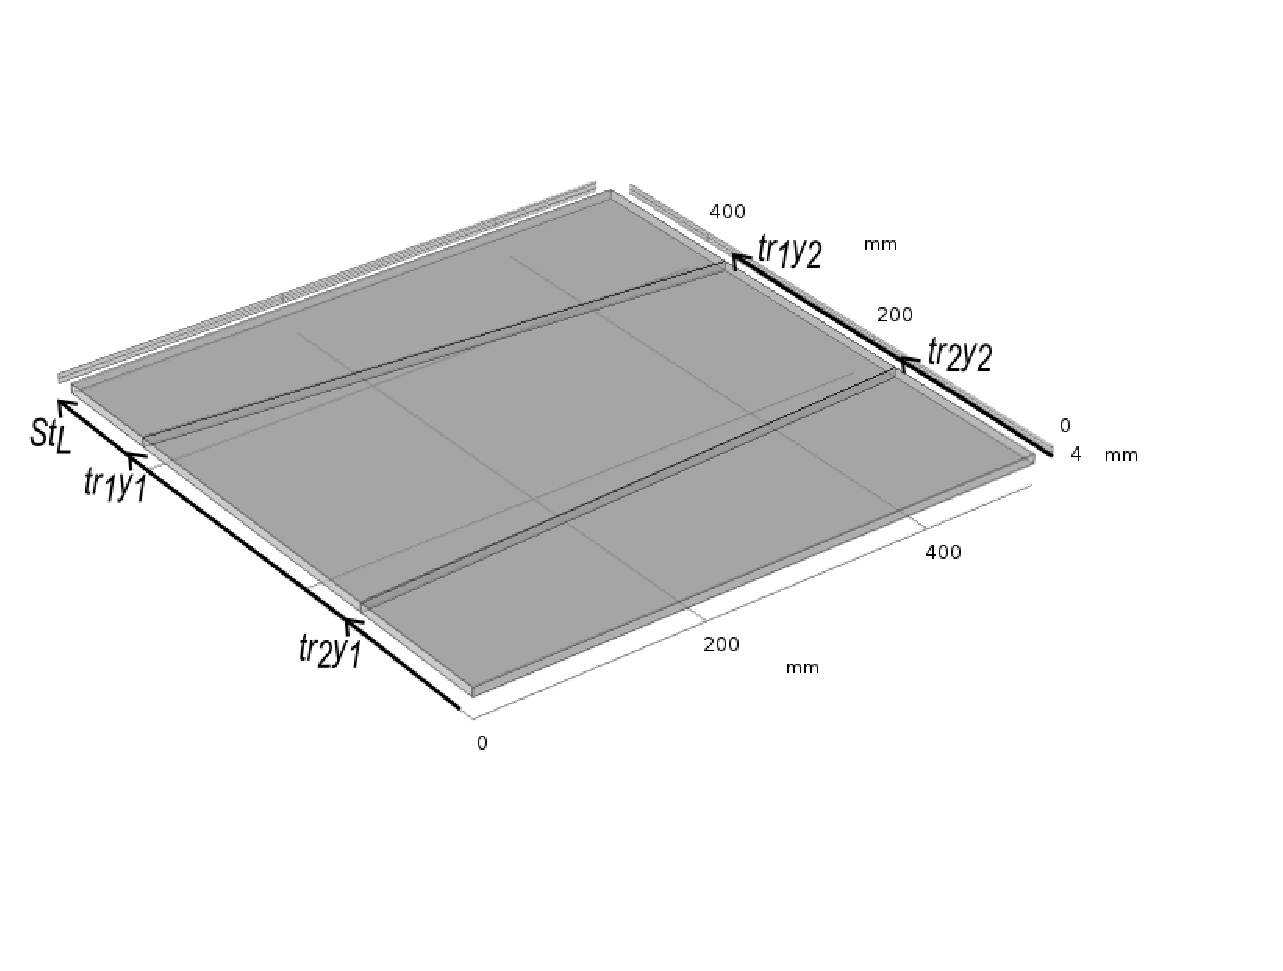
\includegraphics[scale=0.45]{images/StirrerDistances}
\par\end{centering}
\caption{\label{fig: Stirrer_geometry}Stirrer geometry and angle of wings}
\end{figure}
All the parameters and the designated values that are represented
in the figures shown above have been described in Table \ref{tab:Model-parameters-1}.
\par\end{flushleft}

\begin{table}[H]
\caption{Model parameters and values\label{tab:Model-parameters-1}}
\begin{tabular}{cllccccc}
 &  &  &  &  &  &  & \tabularnewline
\hline 
\hline 
Equipment & Parameter &  & Symbol &  & Value &  & Unit\tabularnewline
\hline 
\hline 
Aluminum Chamber & Height &  & $Ch_{H}$ &  & $960$ &  & mm\tabularnewline
 & Width &  & $Ch_{W}$ &  & $790$ &  & mm\tabularnewline
 & Length &  & $Ch_{L}$ &  & $673$ &  & mm\tabularnewline
 &  &  &  &  &  &  & \tabularnewline
Vivaldi Antenna & Height &  & $An_{H}$ &  & $80$ &  & mm\tabularnewline
 & Length &  & $An_{L}$ &  & $110$ &  & mm\tabularnewline
 & Thickness &  & $An_{Th}$ &  & $1.5$ &  & mm\tabularnewline
 & Angle in chamber &  & $\gamma$ &  & $45$ &  & degree\tabularnewline
 & Position in x-direction &  & $An_{x,\textrm{pos}}$ &  & $0$ &  & mm\tabularnewline
 & Position in y-direction n &  & $An_{y,\textrm{pos}}$ &  & $0$ &  & mm\tabularnewline
 & Position in z-direction &  & $An_{z,\textrm{pos}}$ &  & $100$ &  & mm\tabularnewline
 & Frequency &  & $f$ &  & $2.1603$ &  & \textsf{$\textrm{G\ensuremath{\textrm{H}_{z}}}$}\tabularnewline
 & Characteristic impedance &  & $Z_{ref}$ &  & $50$ &  & $\Omega$\tabularnewline
 & Voltage &  & $V_{0}$ &  & $7$ &  & V\tabularnewline
 & Substrate thickness &  & $H$ &  & $1.6$ &  & mm\tabularnewline
 &  &  &  &  &  &  & \tabularnewline
Stirrer & Length &  & $St_{L}$ &  & $340$ &  & mm\tabularnewline
 & Width &  & $St_{W}$ &  & $300$ &  & $\textrm{mm}$\tabularnewline
 & Thickness &  & $St_{Th}$ &  & $3$ &  & $\textrm{mm}$\tabularnewline
 & Position in x direction &  & $St_{x,\textrm{pos}}$ &  & $0$ &  & mm\tabularnewline
 & Position in y direction &  & $St_{y,\textrm{pos}}$ &  & $0$ &  & mm\tabularnewline
 & Position in z direction &  & $St_{z,\textrm{pos}}$ &  & $860$ &  & mm\tabularnewline
 & Angle of stirrer wings &  & $\alpha_{1}$ &  & $60$ &  & degree\tabularnewline
 & Angle of stirrer wings &  & $\alpha_{2}$ &  & $40$ &  & $\textrm{degree}$\tabularnewline
 & Angle in relation to ceiling &  & $\beta$ &  & $10$ &  & $\textrm{degree}$\tabularnewline
 & Distance 1 &  & $tr_{1}y_{1}$ &  & $240$ &  & $\textrm{mm}$\tabularnewline
 & Distance 2 &  & $tr_{1}y_{2}$ &  & $100$ &  & $\textrm{mm}$\tabularnewline
 & Distance 3 &  & $tr_{2}y_{1}$ &  & $240$ &  & mm\tabularnewline
 & Distance 4 &  & $tr_{2}y_{2}$ &  & $100$ &  & mm\tabularnewline
\hline 
\end{tabular}
\end{table}


\subsection{Variation of the stirrer shape and quantity in an ERC}

\subsubsection{Simulation Performance}

As mentioned in the previous chapter, both the shape and the number
of stirrers are crucial to achieve a statistically uniform and isotropic
field. First, the shape of a stirrer is considered and changed. To
do this, all parameters in the table \ref{tab:Model-parameters-1}
are left at the same value except for the four distance. These values
change the shape of the wings. The model was simulated for $40$ stirrer
positions and $9$ degree steps and measurements were recorded from
$9$ different points spaced out within the chamber. From these points
a value of the electric field in both imaginary and rael parts in
each direction was measured and averaged over 9 points. The following
distribution of these fields is displayed for distance in table \ref{tab:Model-parameters-1}.

\begin{figure}[H]
\noindent \begin{raggedright}
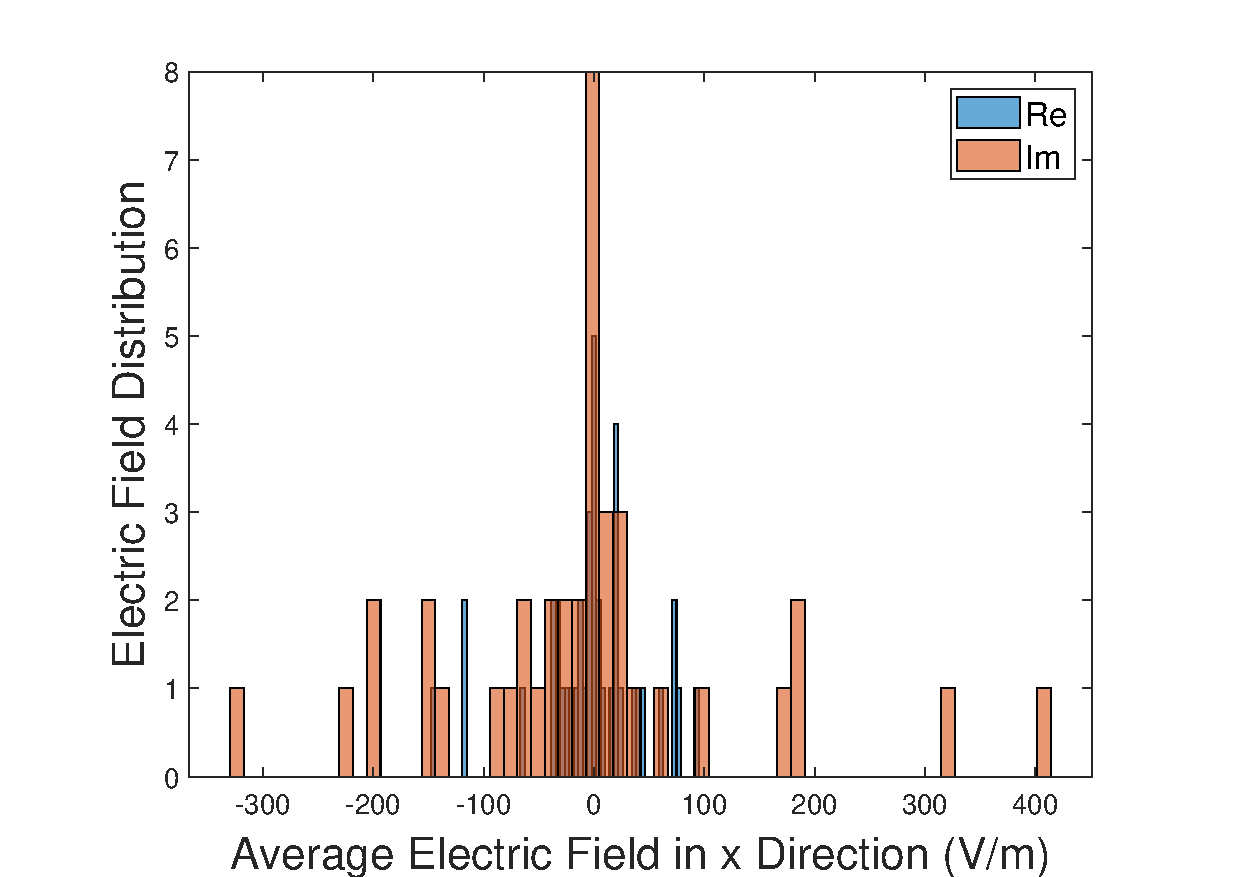
\includegraphics[bb=53bp 0bp 550bp 425bp,clip,scale=0.32]{images/1StirrerXdir}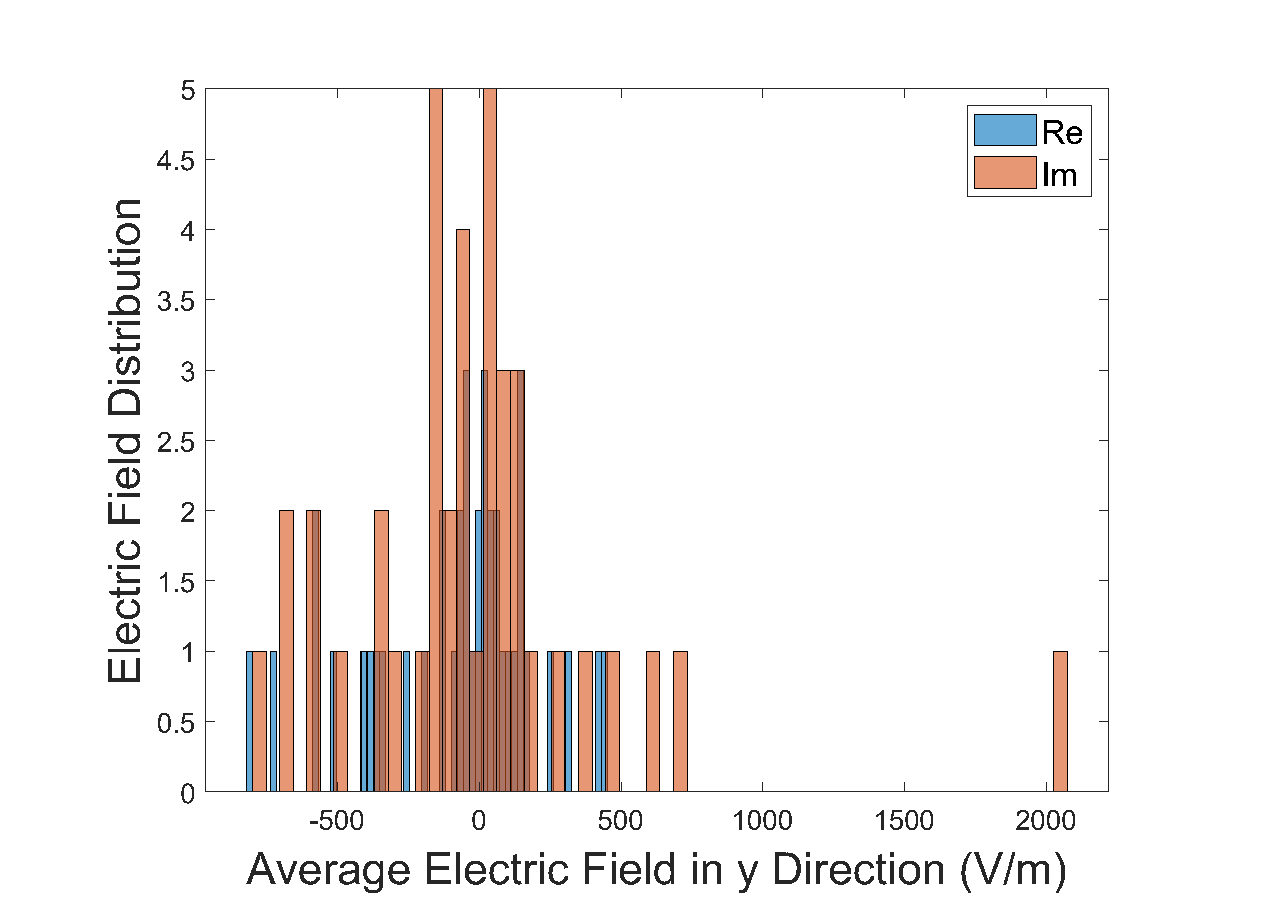
\includegraphics[bb=43bp 0bp 530bp 421bp,clip,scale=0.32]{images/1StirrerYdir}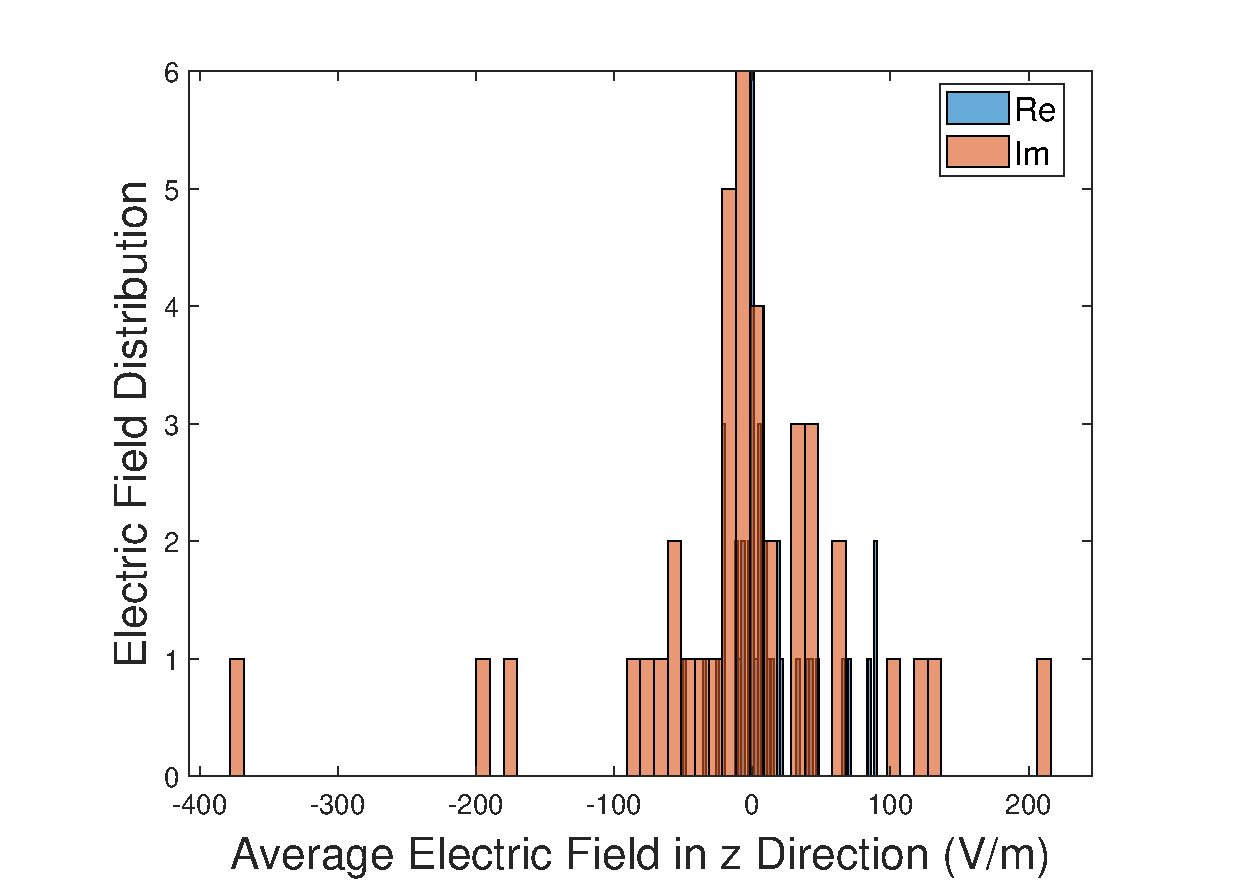
\includegraphics[bb=40bp 0bp 540bp 425bp,clip,scale=0.32]{images/1StirrerZdir}
\par\end{raggedright}
\caption{\label{fig:simulation_noOpt}Distribution of the average electric
field}
\end{figure}
Resulting from these electric field distributions, the following $P$-values
were determined in Matlab.

\begin{table}[H]
\caption{\label{tab:P-value_noOPt}Resulting $P$-values of the simulation}

\centering{}%
\begin{tabular}{lcccccc}
 &  &  &  &  &  & \tabularnewline
\hline 
\hline 
Average Electric Field Distribution &  & Direction &  & $P$-value &  & $\sigma$ in V/m\tabularnewline
\hline 
\hline 
Real Part &  & $x$ &  & $0.0078$ &  & $48,75$\tabularnewline
 &  & $y$ &  & $0.0505$ &  & $296,54$\tabularnewline
 &  & $z$ &  & $0.0036$ &  & $34,25$\tabularnewline
 &  &  &  &  &  & \tabularnewline
Imaginary Part &  & $x$ &  & $0.0030$ &  & $133,67$\tabularnewline
 &  & $y$ &  & $2.3123\times10^{-5}$ &  & $464,76$\tabularnewline
 &  & $z$ &  & $1.0217\times10^{-4}$ &  & $92,64$\tabularnewline
\hline 
\end{tabular}
\end{table}
The $P$-values from the simulation with the initial stirrer geometry
do not reach the requirements discussed in the previous chapter. Consequently,
these results lead to the construction of a new stirrer whose geometry
allows for higher $P$-values. Thus, this issue will be considered
as an optimization problem, that will be solved through the use of
genetic algorithms.

\subsubsection{Performance of the optimized stirrer geometry}

The following parameters listed in Table \ref{tab:Solution-space-for-1}
are the solution spaces for the algorthms, where the range and step
size build the resolution of this space.
\begin{flushleft}
\begin{table}[H]
\caption{\label{tab:Solution-space-for-1}Solution space for genetic algorithms}

\centering{}%
\begin{tabular}{lcccccccc}
 &  &  &  &  &  &  &  & \tabularnewline
\hline 
\hline 
Symbol &  & Range &  & Step size &  & Unit &  & Description\tabularnewline
\hline 
$tr_{1}y_{1}$ &  & $\left[\begin{array}{cc}
240 & 330\end{array}\right]$ &  & $9$ &  & mm &  & distance\tabularnewline
$tr_{1}y_{2}$ &  & $\left[\begin{array}{cc}
240 & 330\end{array}\right]$ &  & $9$ &  & mm &  & distance\tabularnewline
$tr_{2}y_{1}$ &  & $\left[\begin{array}{cc}
10 & 100\end{array}\right]$ &  & $9$ &  & mm &  & distance\tabularnewline
$tr_{2}y_{2}$ &  & $\left[\begin{array}{cc}
10 & 100\end{array}\right]$ &  & $9$ &  & mm &  & distance\tabularnewline
\hline 
\end{tabular}
\end{table}
\par\end{flushleft}

The objective function that we used is the Shapiro-Wilk-Test value
$P$ for the real and imaginary average electric field in each of
the three directions in terms of the different parameters or distance.

\begin{equation}
F_{P}=\sqrt{\overset{6}{\underset{i=1}{\sum}}\left|P_{i}\left(tr_{1}y_{1},tr_{1}y_{2},tr_{2}y_{1},tr_{2}y_{2}\right)-\mathbb{\mathrm{1}}\right|^{2}}\rightarrow\mathrm{min}.
\end{equation}


\subsubsection{Performance of the optimized shape for three stirrers in chamber}
\begin{flushleft}
In Fig.\ref{fig:MVK_dreiStr}, we observe the reverberation chamber
with three stirrer whose geometries have will later be optimized.
\begin{figure}[H]
\centering{}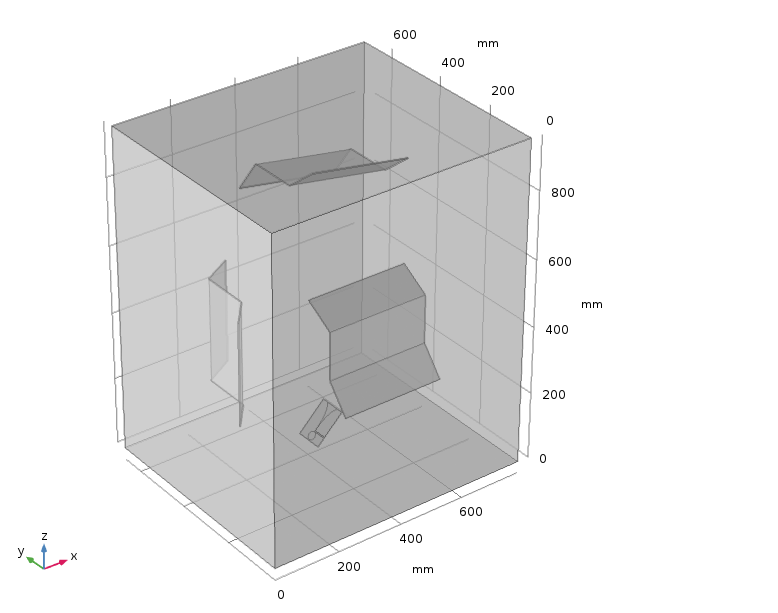
\includegraphics[bb=-67.5578bp 0bp 502.931bp 460bp,clip,scale=0.7]{images/3stirrers}\caption{\label{fig:MVK_dreiStr}Setup of the resonance chamber with three
stirrers, see Table \ref{tab:Model-parameters-3} for their postions}
\end{figure}
 The positions of all three stirrers are listed in Table \ref{tab:Model-parameters-3}.
\par\end{flushleft}

\begin{table}[H]
\centering{}\caption{Model parameters and values\label{tab:Model-parameters-3}}
\begin{tabular}{cllccccc}
 &  &  &  &  &  &  & \tabularnewline
\hline 
\hline 
Equipment & Parameter &  & Symbol &  & Value &  & Unit\tabularnewline
\hline 
Stirrer 1 & Position in x direction &  & $St_{x,1}$ &  & $0$ &  & mm\tabularnewline
 & Position in y direction &  & $St_{y,1}$ &  & $0$ &  & mm\tabularnewline
 & Position in z direction &  & $St_{z,1}$ &  & $860$ &  & mm\tabularnewline
Stirrer 2 & Position in x direction &  & $St_{x,2}$ &  & $0$ &  & mm\tabularnewline
 & Position in y direction &  & $St_{y,2}$ &  & $100$ &  & mm\tabularnewline
 & Position in z direction &  & $St_{z,2}$ &  & $0$ &  & mm\tabularnewline
Stirrer 3 & Position in x direction &  & $St_{x,3}$ &  & $100$ &  & mm\tabularnewline
 & Position in y direction &  & $St_{y,3}$ &  & $0$ &  & mm\tabularnewline
 & Position in z direction &  & $St_{z,3}$ &  & $0$ &  & mm\tabularnewline
\hline 
\end{tabular}
\end{table}
The parameters that have been chosen to be optimized are the shape
of the wings for all three stirrers inside the chamber. The newly
formulated fitness function for these selected parameters is

\begin{equation}
F_{P}=\sqrt{\overset{6}{\underset{i=1}{\sum}}\left|P_{i}\left(tr_{11}y_{1},...,tr_{23}y_{2}\right)-1\right|^{2}}\rightarrow\mathrm{min}.
\end{equation}

A new solution space for the three stirrers is specified in Table
\ref{tab:Solution-space-for-3}.
\begin{flushleft}
\begin{table}[H]
\caption{\label{tab:Solution-space-for-3}Solution space for genetic algorithms}

\centering{}%
\begin{tabular}{lllcccccccc}
 &  &  &  &  &  &  &  &  &  & \tabularnewline
\hline 
\hline 
Equipment &  & Symbol &  & Range &  & Step size &  & Unit &  & Description\tabularnewline
\hline 
Stirrer 1 &  & $tr_{11}y_{1}$ &  & $\left[\begin{array}{cc}
240 & 330\end{array}\right]$ &  & $9$ &  & mm &  & stirrer wing distance 1\tabularnewline
 &  & $tr_{11}y_{2}$ &  & $\left[\begin{array}{cc}
240 & 330\end{array}\right]$ &  & $9$ &  & mm &  & stirrer wing distance 2\tabularnewline
 &  & $tr_{21}y_{1}$ &  & $\left[\begin{array}{cc}
10 & 100\end{array}\right]$ &  & $9$ &  & mm &  & stirrer wing distance 3\tabularnewline
 &  & $tr_{21}y_{2}$ &  & $\left[\begin{array}{cc}
10 & 100\end{array}\right]$ &  & $9$ &  & mm &  & stirrer wing distance 4\tabularnewline
Stirrer 2 &  & $tr_{12}y_{1}$ &  & $\left[\begin{array}{cc}
240 & 330\end{array}\right]$ &  & $9$ &  & mm &  & stirrer wing distance 1\tabularnewline
 &  & $tr_{12}y_{2}$ &  & $\left[\begin{array}{cc}
240 & 330\end{array}\right]$ &  & $9$ &  & mm &  & stirrer wing distance 2\tabularnewline
 &  & $tr_{22}y_{1}$ &  & $\left[\begin{array}{cc}
10 & 100\end{array}\right]$ &  & $9$ &  & mm &  & stirrer wing distance 3\tabularnewline
 &  & $tr_{22}y_{2}$ &  & $\left[\begin{array}{cc}
10 & 100\end{array}\right]$ &  & $9$ &  & mm &  & stirrer wing distance 4\tabularnewline
Stirrer 3 &  & $tr_{13}y_{1}$ &  & $\left[\begin{array}{cc}
240 & 330\end{array}\right]$ &  & $9$ &  & mm &  & stirrer wing distance 1\tabularnewline
 &  & $tr_{13}y_{2}$ &  & $\left[\begin{array}{cc}
240 & 330\end{array}\right]$ &  & $9$ &  & mm &  & stirrer wing distance 2\tabularnewline
 &  & $tr_{23}y_{1}$ &  & $\left[\begin{array}{cc}
10 & 100\end{array}\right]$ &  & $9$ &  & mm &  & stirrer wing distance 3\tabularnewline
 &  & $tr_{23}y_{2}$ &  & $\left[\begin{array}{cc}
10 & 100\end{array}\right]$ &  & $9$ &  & mm &  & stirrer wing distance 4\tabularnewline
\hline 
\end{tabular}
\end{table}
\par\end{flushleft}

\subsection{Variation of geometrie and amount of built-in objects in an ERC}

\subsubsection{Simulation of using different geometric objects in ERC}
\begin{flushleft}
Arrays of the chosen two geometric objects, half spheres and cones,
were inserted inside the chamber cavity \ref{fig:MVK_geo} with parameters
specified in Table \ref{tab:param_geo}. These equidistant objects
are of the same radius (R= 120 mm) and are modeled as such in order
to ultimately compare the values of each simulation and, thus, posses
the representation with the better results. 
\begin{figure}[H]
\centering{}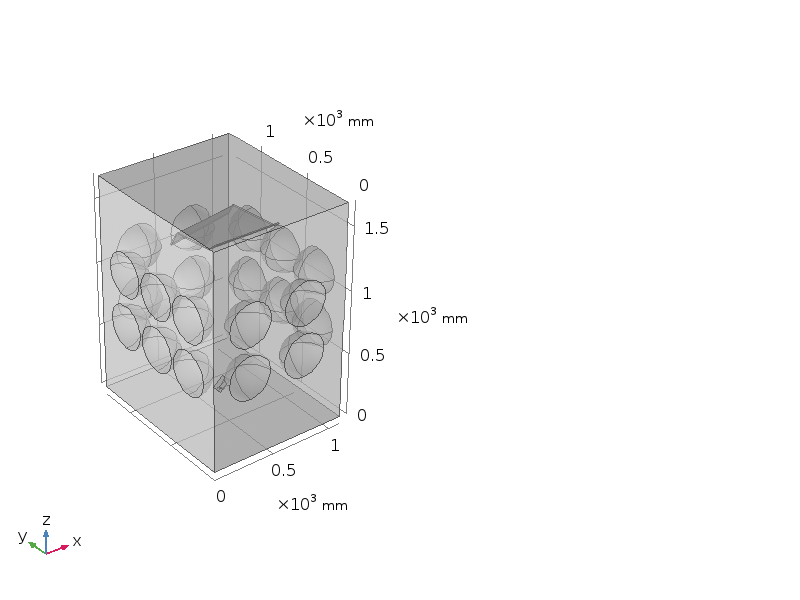
\includegraphics[bb=-60bp 0bp 375bp 435bp,clip,scale=0.6]{images/Kugel2}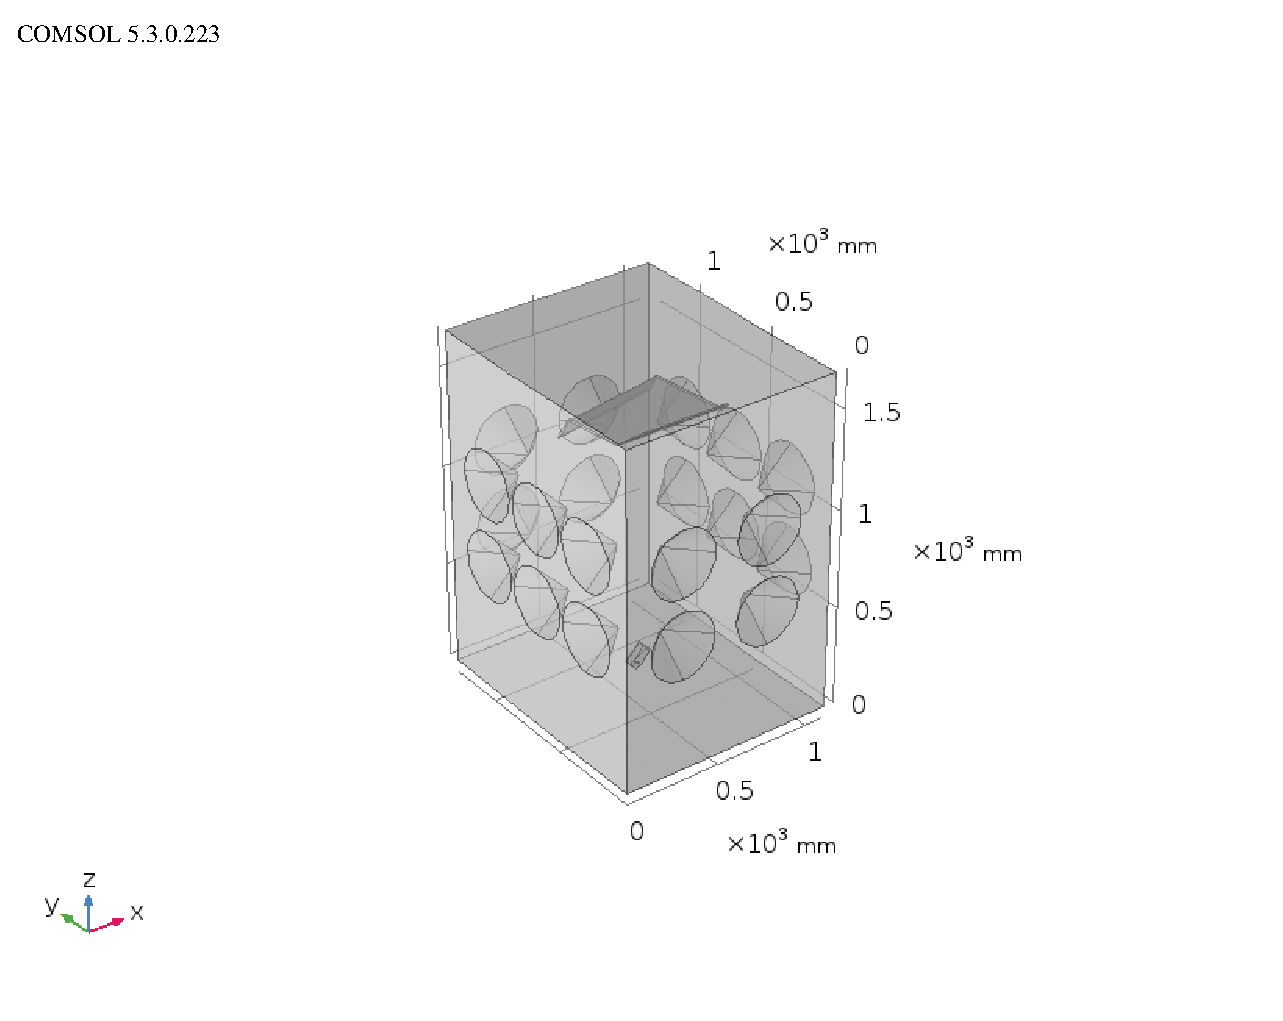
\includegraphics[bb=172.5bp 7.5bp 487.5bp 435bp,clip,scale=0.6]{images/Kegel1}\caption{\label{fig:MVK_geo}Electromagnetic resonance chamber with half spheres
and cones plaiced inside with the same distance between each other}
\end{figure}
\par\end{flushleft}

\begin{flushleft}
The dimensions of the chosen objects, as seen in Table \ref{tab:param_geo},
were similarly selected in order to definitively say which geometry
produces more satisfactory results.
\begin{table}[H]
\caption{\label{tab:param_geo} Dimensions of used geometric objects}

\centering{}%
\begin{tabular}{lcccccc}
 &  &  &  &  &  & \tabularnewline
\hline 
\hline 
Symbol &  & Optimized Values &  & Unit &  & Description\tabularnewline
\hline 
$Rad_{Sph}$ &  & $120$ &  & mm &  & radius of the sphere\tabularnewline
$Rad_{Con}$ &  & $120$ &  & mm &  & radius of the cone\tabularnewline
$Con_{H}$ &  & $120$ &  & mm &  & cone height\tabularnewline
\hline 
\end{tabular}
\end{table}
\par\end{flushleft}

\bibliographystyle{bibtex-daten/unsrtdin}
\bibliography{bibtex-daten/bachelorarbeit-info}

\end{document}
